\documentclass{standalone}
\usepackage{tikz}
\begin{document}
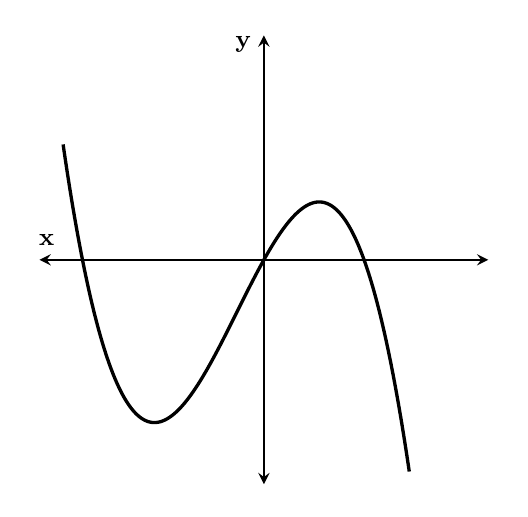
\begin{tikzpicture}[color=black, >=stealth, scale=0.6]
  % Axes (unlabeled scale)
  \draw[<->, thick] (-4.75,0) -- (4.75,0);
  \draw[<->, thick] (0,-4.75) -- (0,4.75);
  \node[font=\small\bfseries] at (-4.6,0.42) {x};
  \node[font=\small\bfseries] at (-0.44,4.55) {y};
  % Cubic, negative leading coefficient: zeros at -3.84, 0 and 2.12
  \begin{scope}
    \clip (-5,-4.85) rectangle (5,4.85);
    \draw[line width=1.2pt, smooth, samples=200, domain=-4.25:3.08]
      plot (\x, {-0.22*\x*(\x + 3.84)*(\x - 2.12)});
  \end{scope}
\end{tikzpicture}
\end{document}
